\documentclass[hyperref={unicode}]{beamer}
%
% Choose how your presentation looks.
%
% For more themes, color themes and font themes, see:
% http://deic.uab.es/~iblanes/beamer_gallery/index_by_theme.html
%
\mode<presentation> {
	\usetheme{Berkeley}      % or try Darmstadt, Madrid, Warsaw, ...
	\usecolortheme{wolverine} % or try albatross, beaver, crane, ...
	\usefonttheme{default}  % or try serif, structurebold, ...
	\setbeamertemplate{navigation symbols}{}
%	\setbeamertemplate{caption}[numbered]
	\setbeamertemplate{caption}{\raggedright\insertcaption\par}
	% Numbered bibiolgraphy items
%	\setbeamertemplate{bibliography item}{\insertbiblabel}
}

\usepackage[utf8]{inputenc}
\usepackage[english]{babel}
\usepackage[T1]{fontenc}
\usepackage{csquotes,lmodern,silence}

\usepackage{textpos}
%\usepackage[style=numeric,backend=biber]{biblatex}

%\WarningFilter{biblatex}{Patching footnotes failed}

% Remove small caps warning
%\renewcommand\mkbibacro[1]{{\footnotesize\MakeUppercase{#1}}}

%\addbibresource{bibliography.bib}
\graphicspath{{figures/}}

\title[Linux Boards]{Viacúčelový systém merania elektrického výkonu dodávaný elektrickými zásuvkami}
\author{Peter Babič}
\institute{Technická Univerzita v Košiciach \\ Počítačové Modelovanie, Ing.}
\date{24.05.2016}

\begin{document}

\addtobeamertemplate{frametitle}{}{%
	\begin{textblock*}{1cm}(.75\textwidth,-1.45cm)
		
\includegraphics[height=1.25cm,width=1.25cm]{logo-tu}
	\end{textblock*}
	\begin{textblock*}{1cm}(.90\textwidth,-1.45cm)
		
\includegraphics[height=1.25cm,width=1.25cm]{logo-fei}
	\end{textblock*}
}

\section{Úvod}

\begin{frame}{\phantom{A}}
	\maketitle
\end{frame}

\subsection{Podnety}
\label{sub:Podnety}

\begin{frame}{Podnety práce}
	\begin{itemize}
		\item Môžeme si dovoliť plytvať elektrickou energiou?
		\item Prečo merať výkon už pri zásuvke?
		\item Čo chýba meračom už zavedeným na trhu?
	\end{itemize}

	% \vskip 1cm

	\begin{figure}[htp]
		\centering
		% 
\includegraphics[width=.25\linewidth]{arrow-up}\hfill
		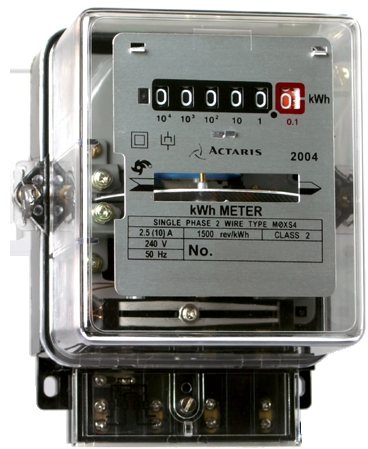
\includegraphics[height=5cm]{analog-power-meter}\hfill
		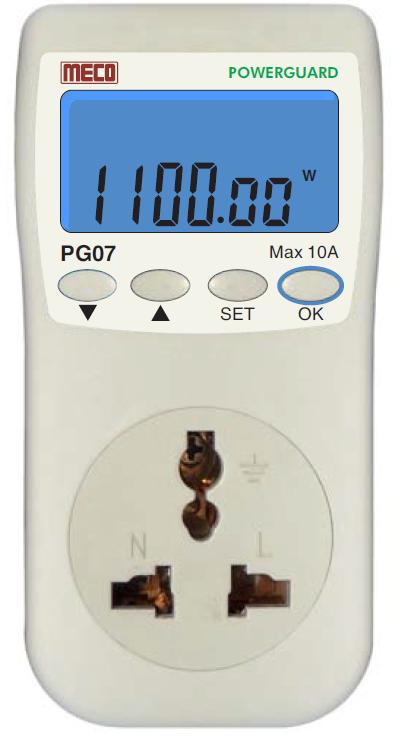
\includegraphics[height=5cm]{digital-plug-meter}
		% \caption{default}
		% \label{fig:figure3}
	\end{figure}

\end{frame}




\section{Záver}

\begin{frame}{Otázky?}
	\centering
	{\Large Ďakujem}
\end{frame}



\end{document}
